% !TeX spellcheck = en_GB
\documentclass[usenames,dvipsnames,aspectratio=169]{beamer}
\usetheme{Szeged}
\usecolortheme{beaver}
\usepackage{tikz}
\setbeamertemplate{navigation symbols}{}
\usepackage{xcolor}

% \addbibresource{../VorlageAbschlussarbeit/Vorlage-Abschlussarbeit/Abschlussarbeit.bib}


\title{Web Processing - Standardized GIS Analyses for Cable Route Planning}
\author{Sebastian Heiden}
\institute{Harz University of Applied Sciences}
\date{December 02, 2022}
\begin{document}

    

\begin{frame}[plain]
	\includegraphics[scale=0.21]{3-HSH-Logo-RGB-en.png}
    \maketitle
\end{frame}
%\begin{frame}{Structure}
%    \tableofcontents    
%\end{frame}

\section{Topic and Motivation}
\begin{frame}{Topic and Motivation}
\begin{columns}[T] % align columns
\begin{column}{.68\textwidth}
	Topic
	\begin{itemize}
		\item route planning, e.g. connection of offshore wind farms to the power grid
		{\item \color{gray} conflicts with land usage, land coverage, regulation}
		\item routing cables from landing point to final position
		\item offer a standard web service for the routing
	\end{itemize}
	\vspace{0.5cm}
	
	\color{gray} Motivation
	\begin{itemize}
	\color{gray}
		\item Energy Security
		\item Contribution to important real world problems
	\end{itemize}
\end{column}%
\hfill
\begin{column}{.28\textwidth}
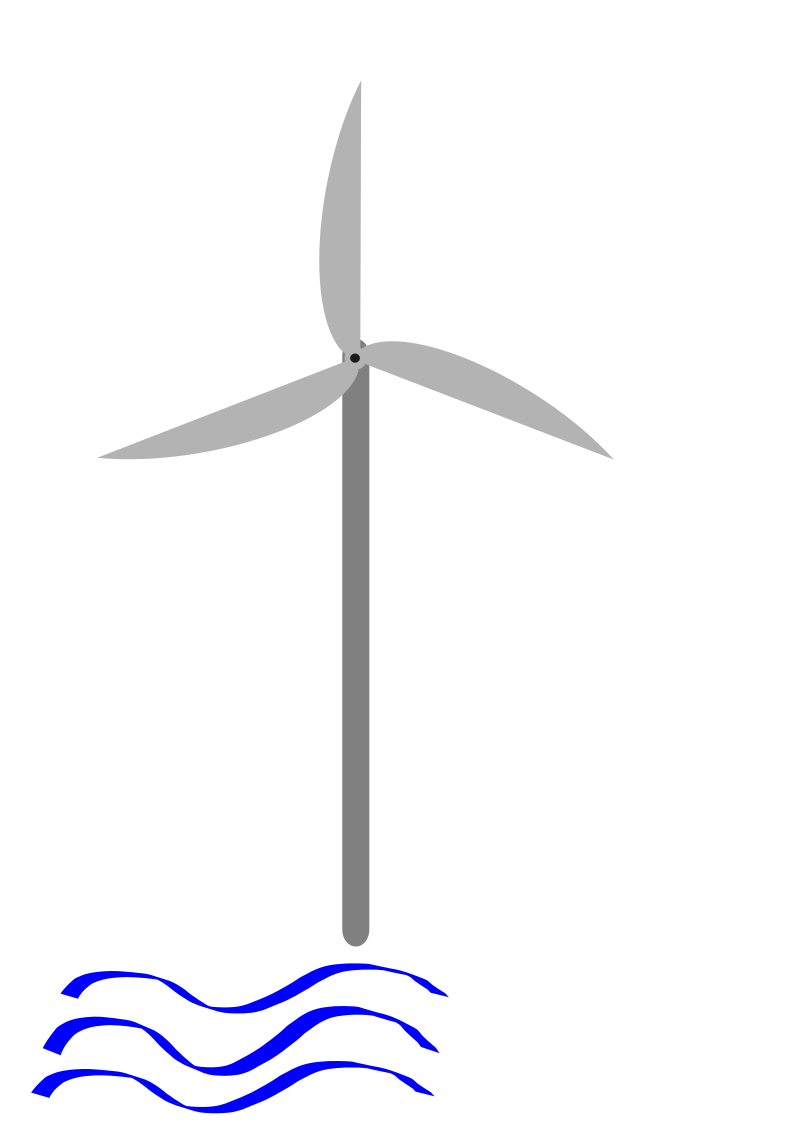
\includegraphics[scale=0.2]{icon_offshore_wind_turbine.png}
\end{column}%
\end{columns}
\end{frame}

\section{Timetable}
\begin{frame}{Timetable}
\begin{center}
	\begin{small}
	\begin{tabular}{  c  c l }
		
		  Start Date & End Date &  \hspace{2.5mm}\\ 
		 \hline  

		09/23/2022 & 					& \hspace{2.5mm} \color{gray}{Project Start}\\
		09/23/2022 & 10/10/2022 	&  \hspace{2.5mm} \color{gray}{Initial Literature Study}\\
		10/01/2022 & 10/23/2022 	&  \hspace{2.5mm} \color{gray}{Initial Data Search}\\
		\hline  
		10/14/2022 & 					& \hspace{2.5mm} \color{gray}{Kick-Off Presentation}\\

		10/16/2022 & 10/28/2022 	&  \hspace{2.5mm} \color{gray}{Data Conversion/Costs/test execution}\\
		10/28/2022 & 12/31/2022 	&  \hspace{2.5mm} \color{red}{provide WPS/implement LCP}\\
		\hline  
		12/02/2022 & 					& \hspace{2.5mm} \color{gray}{Midterm  Presentation}\\
		
		12/14/2022 & 02/01/2022 	& \hspace{2.5mm} Optimization/Research Issue\\
		02/01/2022 & 					& \hspace{2.5mm} Feature Freeze \\ 

		02/01/2022 & 02/28/2023 	& \hspace{2.5mm} Finalizing Report\\ 
		\hline  
		02/28/2023 & 					& \hspace{2.5mm} Submission  \\
		03/15/2023 & 					& \hspace{2.5mm} Final Presentation  \\
		   
	\end{tabular}
	\end{small}
\end{center}
\end{frame}


\section{Create the cost raster}
\begin{frame}{Get Land coverage/ usage planning}
	%Area Under Study:
	%\begin{itemize}
	%	\item Cuxhaven county
	%	\item Osterholz county
	%\end{itemize}
	
	\begin{tabular}{ l  p{75mm} }
		Datatype & Sources\\
		\hline 
		Protected Areas 	& German Environment Agency\footnote{https://geodienste.bfn.de/schutzgebiete?lang=de}\\
		land usage & Federal Agency for Cartography and Geodesy\footnote{https://gdz.bkg.bund.de/index.php/default/open-data.html} \\
		planning land usage & 'Metropolplaner' (Planing data Lower Saxony \& Bremen)\footnote{https://metropolplaner.de/metropolplaner/}\\
		Houses (Level of Detail 1) &State Office for Geoinformation and \newline Land Surveying of Lower Saxony\footnote{https://opengeodata.lgln.niedersachsen.de/}\\
		transformers, power lines  & OpenStreetMap\\
	\end{tabular}
\end{frame}


\begin{frame}{Rasterization}
	\begin{itemize}
		\item vector (point, line, polygon) --> raster
		\item all touched <-- false
	\end{itemize}
	\vspace{5.0mm}
	\resizebox{11cm}{!}{
	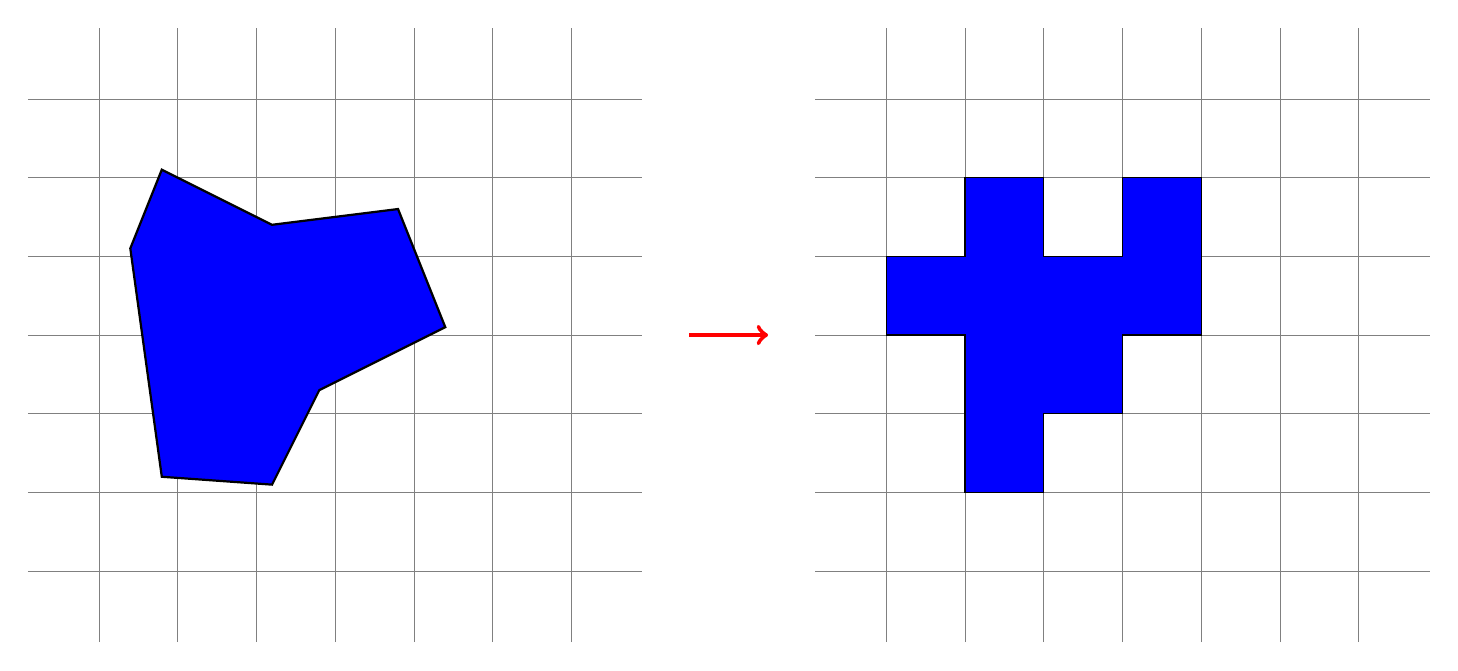
\begin{tikzpicture}
	\draw[step=1cm,gray,very thin] (-1.9,-1.9) grid (5.9,5.9);
	\draw[fill=blue, thick] (-0.2, 0.2)--(-0.6, 3.1)--(-0.2,4.1)--(1.2,3.4)--(2.8,3.6)--(3.2, 2.6)--(3.4, 2.1)--(1.8,1.3)--(1.2, 0.1)--cycle;
	
	\draw[ultra thick,->, red] (6.5, 2) -- (7.5, 2);
	
	\draw[step=1cm,gray,very thin] (8.1,-1.9) grid (15.9,5.9);
	\draw[fill=blue] (10,0)--(10,2)--(9,2)--(9,3)--(10,3)--(10,4)--(11,4)--(11,3)--(12,3)--(12,4)--(13,4)--(13,2)--(12,2)--(12,1)--(11,1)--(11,0)--cycle;
	\end{tikzpicture}
}
\end{frame}


\begin{frame}{Rasterization}
	\begin{itemize}
		\item vector (point, line, polygon) --> raster
		\item all touched <-- true
	\end{itemize}
	\vspace{5.0mm}
	\resizebox{11cm}{!}{
	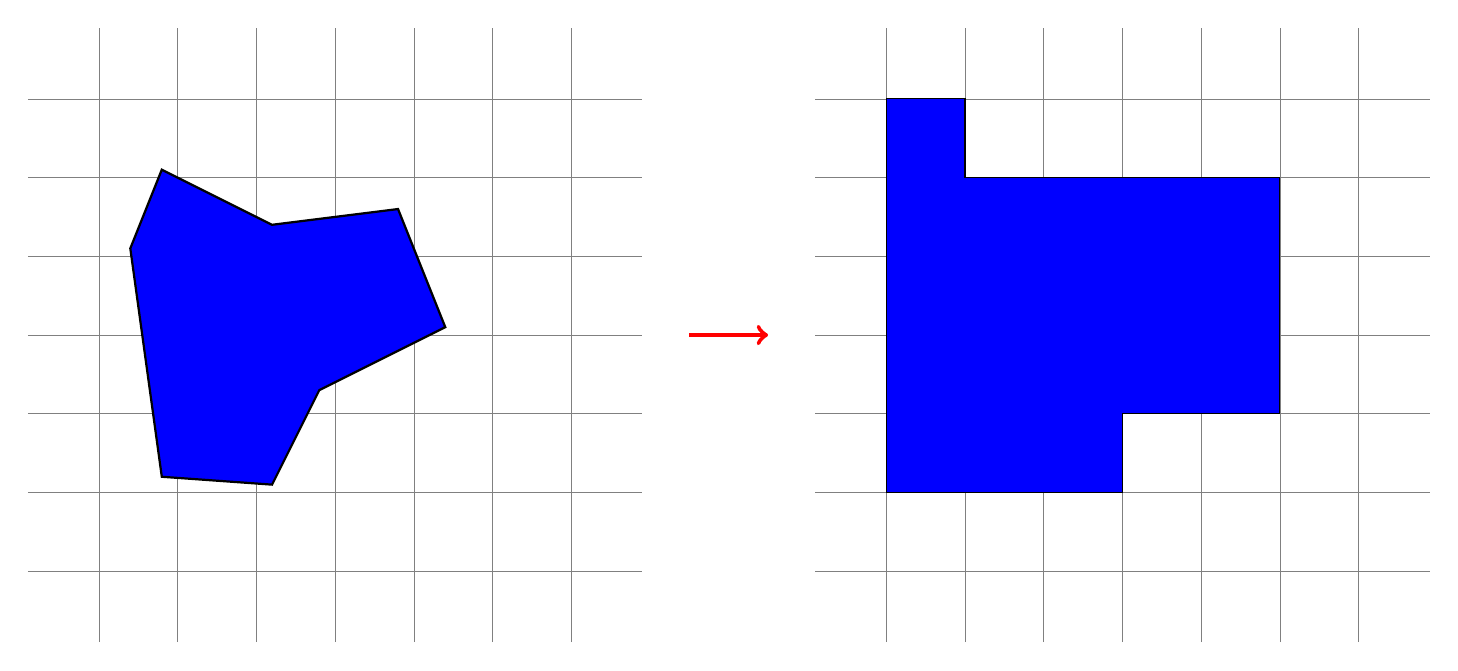
\begin{tikzpicture}
	\draw[step=1cm,gray,very thin] (-1.9,-1.9) grid (5.9,5.9);
	\draw[fill=blue, thick] (-0.2, 0.2)--(-0.6, 3.1)--(-0.2,4.1)--(1.2,3.4)--(2.8,3.6)--(3.2, 2.6)--(3.4, 2.1)--(1.8,1.3)--(1.2, 0.1)--cycle;
	
	\draw[ultra thick,->, red] (6.5, 2) -- (7.5, 2);

	\draw[step=1cm,gray,very thin] (8.1,-1.9) grid (15.9,5.9);
	\draw[fill=blue] (9,0)--(9,5)--(10,5)--(10,4)--(14,4)--(14,1)--(12,1)--(12,0)--cycle;
	\end{tikzpicture}
	}
\end{frame}



\begin{frame}{Costs and Configuration}
	Configuration
	\begin{itemize}
		\item resolution, all touched
		\item calculate by layer:
		\begin{itemize}
			\item filtering by attribute values
			\item buffering by value or/and attribute value
		\end{itemize}
		\item cost calculation: maximum of al layers
	\end{itemize}

	\vspace{5.0mm}
	\begin{tabular}{ l  r  l }
	Cost Level & Cost (numeric) &  Example\\
	\hline
	Prohibited & 500					& National Parks, Buildings \\
	strongly Restricted & 10 	& Bird Sanctuary \\
	Restricted & 5	& industrial areas \\
	No Restriction & 0.5					& \color{green}{default}\\
	Preferential & 0.1					& power grid, motorways buffers\\
\end{tabular}

\end{frame}

\begin{frame}{Cost Raster}
	\begin{columns}[T] % align columns
		\begin{column}{.48\textwidth}
			\begin{figure}[htb]
				\includegraphics[scale=0.2]{../results/images/result_res_100_all_touched_False.png}
				\caption{100 m Resolution with all touched false.}
			\end{figure}
		\end{column}
		\begin{column}{.48\textwidth}
			
		\end{column}
	\end{columns}
\end{frame}

\begin{frame}{Cost Raster}
	\begin{columns}[T] % align columns
		\begin{column}{.48\textwidth}
			\begin{figure}[htb]
				\includegraphics[scale=0.2]{../results/images/result_res_100_all_touched_False.png}
				\caption{100 m Resolution with all touched false.}
			\end{figure}
		\end{column}
		\begin{column}{.48\textwidth}
			\begin{figure}[htb]
				\includegraphics[scale=0.2]{../results/images/result_res_100_all_touched_True.png}
				\caption{100 m Resolution with all touched true.}
			\end{figure}
		\end{column}
	\end{columns}
\end{frame}

\section{web processing server}
\begin{frame}{web processing server}
	\begin{itemize}
		\item goal: calculate path from cost with web service
		\item current: 
		\begin{itemize}
			\item testing pywps\footnote{https://pywps.readthedocs.io/en/latest/index.html}
			\item cost path (open Dijkstra implementation - QGIS-plugin)\footnote{https://github.com/Gooong/LeastCostPath}
		\end{itemize}
	\end{itemize}
\end{frame}


\end{document}
